\documentclass[12pt]{article}
\usepackage{frExamplee}
\usepackage{booktabs}       % professional-quality tables
\usepackage{amsfonts}       % blackboard math symbols
\usepackage{amsmath}
\usepackage{enumitem}
\usepackage{listings}
\lstset{
    language=Python,
    basicstyle=\scriptsize\ttfamily,
    keywordstyle=\color{blue},
    commentstyle=\color{green!50!black},
    stringstyle=\color{red},
    showstringspaces=false,
    numbers=left,
    numberstyle=\footnotesize,
    numbersep=5pt,
    frame=single,
    breaklines=true,
    breakatwhitespace=true,
    tabsize=4,
    captionpos=b
}
\usepackage{amssymb}
\usepackage{graphicx}
\usepackage{csquotes}
\usepackage[backend=biber, style=ieee,]{biblatex}
\usepackage{setspace}
\usepackage[usenames, dvipsnames]{xcolor}
\usepackage{xspace}
\usepackage{caption}
\usepackage{subcaption}
\usepackage{multirow}
\usepackage{float}
\usepackage{wrapfig}
\usepackage{placeins}
\usepackage{algpseudocode}
\usepackage{algorithm}
\usepackage{algorithmicx}
\usepackage{hyperref}
\usepackage{setspace}
\usepackage{fancyhdr} 
\fancyhf{}
\cfoot{\thepage}
\pagestyle{fancy}
\renewcommand{\headrulewidth}{0pt}%

\addbibresource{FRtemplates/frExampleRefs.bib}
\title{An Investigation of the Rydberg Constant of Hydrogen and the Emission Spectra of Gases Using a Tri-prism Spectrometer}
\vspace{-15pt}
\author{
Tony Wang \href{https://orcid.org/0009-0009-3015-7192}{
\includegraphics[height=12pt]{figure/orcid.png}}\\
\texttt{1009027447 | wangq330} \\
\texttt{tonyivt.wang@mail.utoronto.ca}\\
\And
Natasha Yang \href{https://orcid.org/12345}{
\includegraphics[height=12pt]{figure/orcid.png}}\\
\texttt{1008975575 | yangx315} \\
\texttt{nxy.yang@mail.utoronto.ca} \\
}
\begin{document}
\maketitle
\begin{abstract}
    This lab report investigates the Rydberg Constant, $R_H$, of hydrogen and identifies an unknown gas based on its emission spectrum. The experiment involves observing the emission spectra of gases in a discharge tube with a tri-prism spectrometer. Using the Hartmann relation method, we first calibrated the spectrometer by fitting its scale reading, $y$, against the wavelengths of hydrogen and helium spectral lines. Through this, we determined the relation to be $y=\frac{1980 \pm 10}{\lambda - (282.8 \pm 0.4)} + (2.02 \pm 0.05)$. The Rydberg constant was then found to be $R_{H} = (1.10 \pm 0.01) \times 10^7 {\rm  m}^{-1} (R_{EH} = 13.6 \pm 0.1 {\rm eV})$ using Johann Balmer's formula and the predicted wavelengths of hydrogen's spectral lines, $\lambda_{\rm pred}$. The results correspond precisely to literature values up to 3 significant figures. Then, we observed the spectrum of an unknown gas and compared its strong spectral lines to known spectra, identifying the gas to be mercury. Finally, we found the separation of the spectral lines in the yellow doublet of sodium to be $569 \pm 3 {\rm  nm}$ and $591 \pm 3 {\rm nm}$. These values differ greatly from reality, demonstrating the limitation of the spectrometer at resolving closely spaced spectral lines. Overall, while our setup works wonders for substances that have reasonably spaced out emission lines, more precision is needed in order to properly measure wavelengths of closely packed lines like in the case of Sodium.
    
\end{abstract}

%------------------------------------------------------
% 7.41 * 10^-7 [m^2/s]
\section{Introduction}
Early investigations into the spectra emitted by excited atoms by Planck, Bohr and Rydberg provided exciting evidence for the development of quantum theory \autocite{PhysRevA.34.5138}. This experiment explores the emission spectra of various gases within discharge tubes. When a high voltage is applied to the tube, electrons collide with gas atoms, causing ionization and excitation. Since vacancies can be created in any electron shell, electrons transitioning to lower energy states emit photons of various discrete wavelengths. This experiment will examine the relationship between these spectral lines and the discrete energy levels within atoms, correlated via the Rydberg Constant.

From the Empirical Rydberg Equation and Bohr's model of a hydrogen atom, we have:
\begin{equation}
    hf=R_{EH}\left(\frac{1}{m^2}-\frac{1}{n^2}\right)=T_m-T_n
    \label{eq:rydberg}
\end{equation}
where $h$ is Planck's Constant, $f$ is frequency, $R_{R,H}=13.6\;[eV]$ is the Rydberg Constant for Hydrogen, $m,n$ are distinct principal quantum numbers and $T_m,T_n$ are their respective energies \autocite{manuall}. Similarly, Balmer found a relationship between the wavelength and the energy levels of hydrogen in the visible spectrum:
\begin{equation}
    \frac{1}{\lambda}=R_H\left(\frac{1}{2^2}-\frac{1}{n^2}\right)
    \label{eq:balmer}
\end{equation}
where $\lambda$ is the wavelength of the spectrum, $R_H$ is $R_{EH}$ expressed in terms of the reciprocal of distance, $[1/m]$, and n is the principal quantum number like in Rydberg's equation. Note that equations (\ref{eq:rydberg},\ref{eq:balmer}) are essentially the same as we can relate them via the energy of a photon, $E=hc/\lambda=hf$, where $c$ is the speed of light. 




\section{Experiment}
\subsection{Apparatus}
\begin{figure}[h!]
    \centering
    \includegraphics[width=0.6\textwidth]{figure/setup.png}
    \caption{Experimental apparatus with equipment labeled.}
    \label{fig:0}
\end{figure}
\subsection{Equipment and Uncertainties}
\begin{itemize}
    \item Tri-prism spectrometer $(\lambda_0=282.8\pm0.4\;[nm])$
    \item Vernier scale $({\rm reading\;accuracy}\pm0.05\;{\rm units})$
    \item Sodium lamp
    \item Set of discharge tubes (hydrogen gas, helium, and unknown gas)
    \item Power supply for the discharge tube
\end{itemize}

\subsection{Method} 
\subsubsection{Calibration of spectrometer}
In this step, we aim to relate $\lambda$ of a spectral line and the vernier scale reading $y$ on the spectrometer. This will allow us to convert the scale reading of unknown spectral lines to corresponding wavelengths, to achieve this, we will be using helium and hydrogen gas tubes and their known spectral line wavelengths. The relationship we will use is the Hartmann dispersion relation: \autocite{manuall}
\begin{equation}
    y=\frac{m}{\lambda-\lambda_0}+b
    \label{eq:hartmann}
\end{equation}
where $y$ is the reading measured on the vernier scale, $\lambda_0$ is given and specific to to instrument, and $m,b$ are constants that can be found by fitting the relationship curve. The procedure is:
\begin{enumerate}
    \item Pop in the Helium tube and turn on the power supply.
    \item Locate the first spectral line and adjust the focus and aperture until the spectral lines as well as the cross-hair are clear.
    \item Adjust the eyepiece position knob until the cross-hair is centred on the line.
    \item Read and record the reading of $y$ on the vernier scale.
    \item Turn the position knob to find other spectral lines and repeat steps 2-4.
    \item Switch the Helium tube to Hydrogen and repeat steps 2-5
\end{enumerate}
\subsubsection{Identification of unknown gas}
\begin{enumerate}
    \item Switch the Hydrogen tube for a mystery tube.
    \item Locate and record the positions of each spectral line.
    \item For each spectral line, use the recorded readings as well as the relationships discovered prior part to calculate their respective wavelengths. Based on the features of the spectral lines, guess which gas is contained in the mystery tube.
\end{enumerate}
\subsubsection{Calculation of Rydberg's Constant}
Using the derived relation in the calibration step, equation (\ref{eq:hartmann}), calculate the wavelengths of hydrogen and subsequently, $R_E$ and $R_{EH}$ with equations (\ref{eq:rydberg},\ref{eq:balmer}).
\subsubsection{Finding the spectral line separation of sodium}
\begin{enumerate}
    \item Turn off the power supply for the discharge tubes and turn on the sodium lamp.
    \item Wait for the lamp to warm up and turn bright yellow. Observe it through the instrument: there should be two very close spectral lines.
    \item Center the cross-hair and attempt to find the separation. Use the $y$ values to find the respective wavelengths of the two lines.
\end{enumerate}

\section{Data and Discussion}

\begin{figure}[h!]
    \centering
    \begin{subfigure}{0.7\textwidth}
        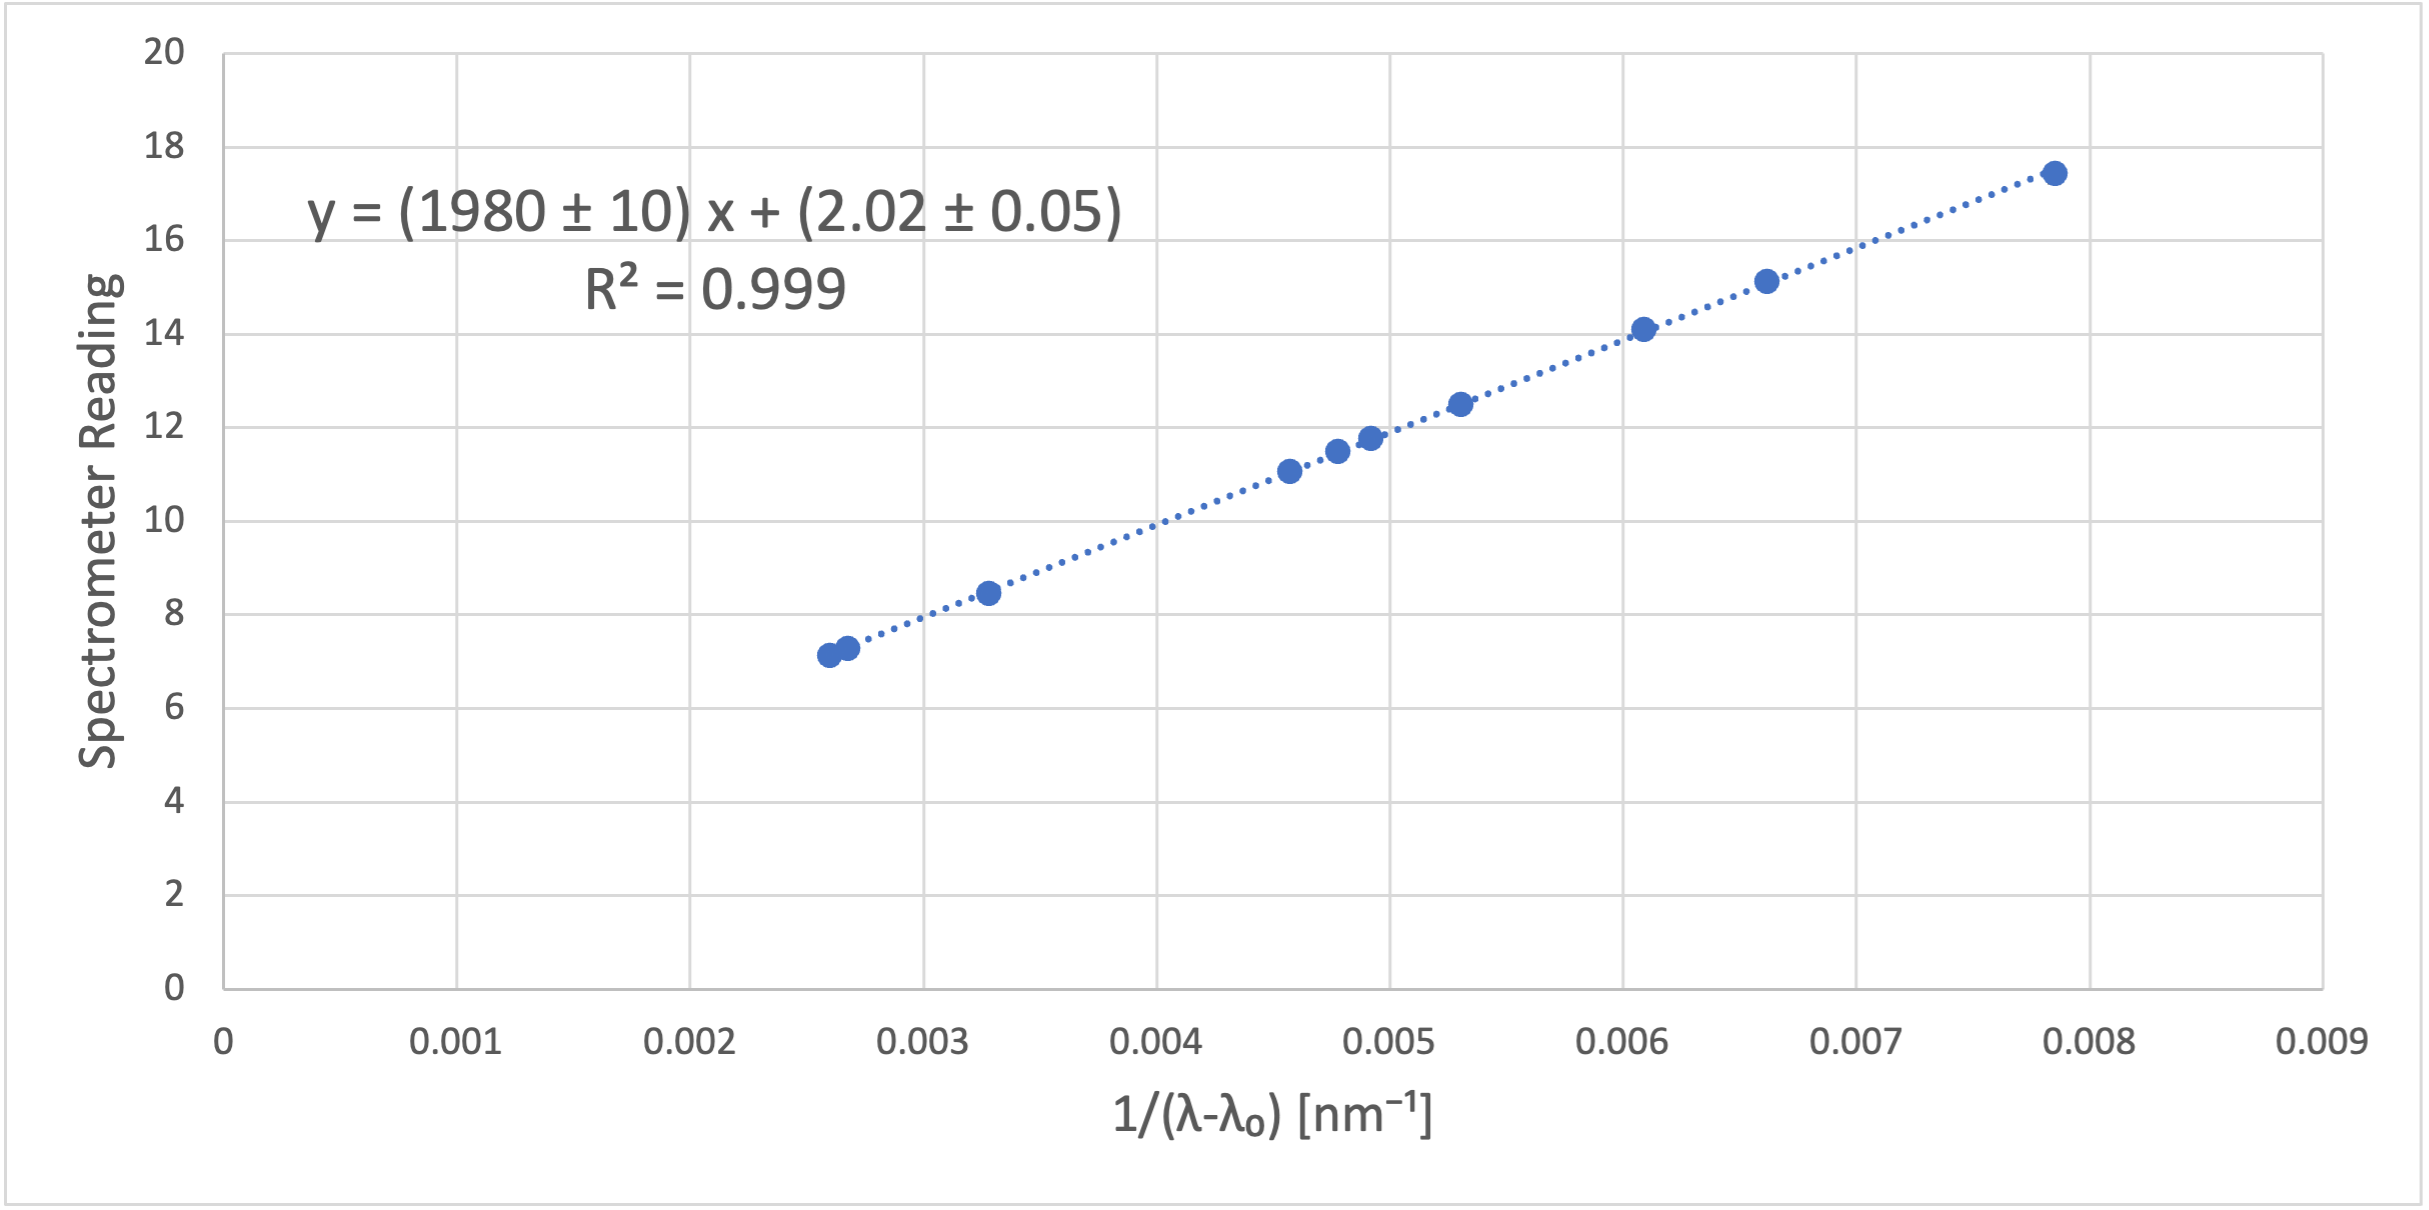
\includegraphics[width=\textwidth]{figure/fit.png}
        \caption{Curve of best fit of \eqref{eq:hartmann}.}
        \label{fig:fit}
    \end{subfigure}
    \hfill
    \begin{subfigure}{0.5\textwidth}
        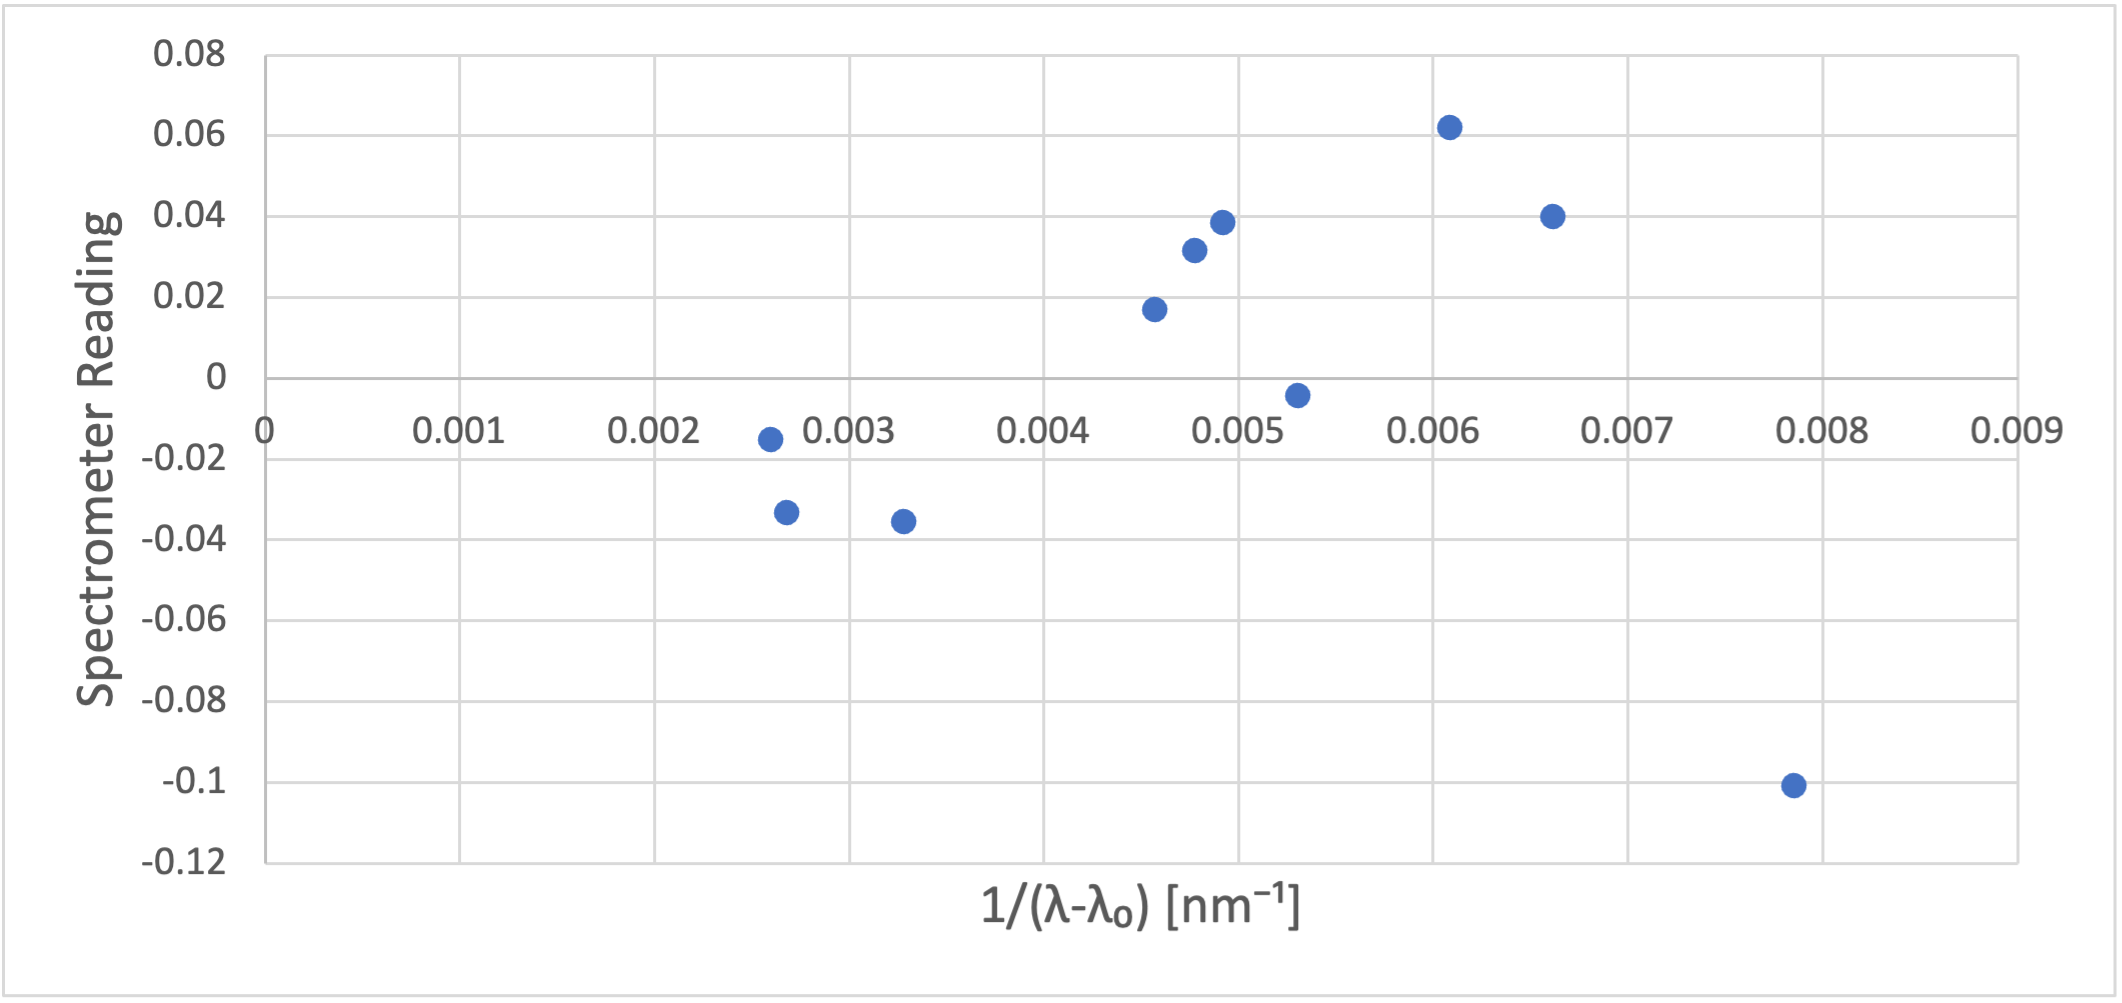
\includegraphics[width=\textwidth]{figure/residuals.png}
        \caption{Residuals of the curve fit of \eqref{eq:hartmann}.}
        \label{fig:residuals}
    \end{subfigure}
    \label{fig:data}
    \caption{Curve fitting of $y(\lambda)$. The goodness of fit criteria are found to be $R^2=0.999$ and $\chi_v^2=1.05$. Uncertainty bars are included but are too small to be visible. Their specific values are in Table \ref{table:calibration}, and are propagated using source uncertainties of the instrument and vernier scale reading error. Propagation formulae are in the appendix.}
\end{figure}
\subsection{Calibration of spectrometer}
Using \eqref{eq:hartmann}, we found the relationship between the spectrometer reading with the wavelength using the equation, 
\begin{equation}
y=m \cdot \frac{1}{\lambda - \lambda_0}+b. 
\label{eq:fit}
\end{equation}

As shown in the curve fitting in Fig.\ref{fig:fit}, the slope and intercept of the line of best fit is 
\begin{equation*}
    m=1980 \pm 10\text{ and }b=2.02 \pm 0.05,
\end{equation*}
respectively.

The uncertainties, goodness of fit criteria and residual plot suggest that the calibration curve is highly accurate. Uncertainties of the fit parameters are less than $2.5\%$ of their respective values, indicating their high precision. Additionally, the line of best fit has a high $R^2$ value of 0.999, which demonstrates that it models the data accurately. As shown in Fig.\ref{fig:residuals}, residuals of the fit are evenly distributed around the x-axis, which suggests that the model represents an unbiased estimation of the relationship. Moreover, the uncertainty estimation is reasonable as the reduced chi-squared, $\chi_v^2$ value is 1.050, which is very close to 1. This assures us that we have accurate tools to identify unknown gases/vapours based on their spectral emission patterns.

However, we observe that most of the error came from the reading uncertainty of the vernier scale. To design the experiment better, errors can almost be completely eliminated by employing a digital micrometre that automatically reads the position of the spectrometer.


\subsection{Identifying an unknown gas}
We were only able to observe four spectral lines emitted by the unknown gas/vapour. While a lot of other fainter lines might have been missed, there is still enough information for us to identify with confidence what the filament of the tube is. Using \eqref{eq:fit} to relate the spectrometer reading to wavelengths and comparing them to known spectra of gases, we found the unknown gas to be mercury as its emission spectra exhibit high similarity to the latter's.

The lines we were able to see and their calculated wavelengths are in Table \ref{table:predicted_wavelengths}. Every wavelength we observed is within aligns closely to that of the lines that are supposed to have high intensity according to the datasheet, where the actual wavelengths are within uncertainty range \autocite{manuall}. The errors are reasonable but not insignificant and are affected mostly by the vernier scale reading error as discussed previously. Also according to the datasheet, there are more than 30 distinct spectral lines emitted by Mercury vapour and we could only identify a minute fraction of them, due to the majority of emitted lines being low in intensity. This has to do with how much light the spectrometer lets through and the photon intensity our retinas can physically receive. This lack of information creates huge uncertainty in differentiating gasses, especially when their emission spectra are similar. To improve the experiment, we can incorporate optics that let in more light emitted by the tubes, safely use a higher voltage to ionize atoms to emit more photons or incorporate an image-capturing device that exposes the fainter spectral lines for longer. The higher the size of the sample of emitted lines we have, the more certain we can be about the identity of a mystery gas. 

\subsection{Computation of the Rydberg Constant}
To calculate the Rydberg constant, we used the given Hydrogen emission wavelengths and rearranged \eqref{eq:balmer} and \eqref{eq:rydberg}to obtain,
\begin{equation}
    R_H=\frac{1}{\lambda} \left( \frac{1}{2^2}-\frac{1}{n^2} \right) ^{-1}.
    \label{eq:rydberg_calculation}
\end{equation}
and
\begin{equation}
    R_{EH}=hf \left( \frac{1}{2^2}-\frac{1}{n^2} \right) ^{-1}=\frac{hc}{\lambda}\left( \frac{1}{2^2}-\frac{1}{n^2} \right) ^{-1}=hcR_H.
    \label{eq:rydberg_calculation}
\end{equation}

By assuming that successive wavelengths correspond to transitions to successive energy levels (e.g. $n=2$, $n=3$, $n=4$, $n=5$ etc.) and averaging the $R_H$ for four wavelengths, we determined the Rydberg constant to be
\begin{equation}
    R_H = 1.10 \pm0.01\times 10^7 \;{\rm m^{-1}}
    \label{eq: R_H}
\end{equation}
or
\begin{equation}
    R_{EH}=13.6\pm0.1\;{\rm eV}.
    \label{eq: R_{EH}}
\end{equation}
These values correspond exactly to the literature values of $R_H$ and $R_{EH}$ rounded to 3 significant figures, indicating the reliability of this experiment \autocite{PhysRevA.34.5138}.
The ionization energy of atomic hydrogen is $1312\;{\rm kJ\cdot mol^{-1}}$ or $13.60\;{\rm eV}$ per atom, which has exactly the same value as Rydberg's constant up to the number of significant figures of our raw data \autocite{PhysRevA.34.5138}. This is expected because in Bohr's model, the energy associated with each principal quantum number is $E_n = \frac{R_H}{n^2}$, so the ionization energy of hydrogen is represented by $E_1 = \frac{R_H}{1^2}=R_H$. Thus in a hydrogen atom, the Rydberg constant $R_{EH}$ represents the amount of energy required to remove an electron from the $n=1$ energy level. The accuracy of our Rydberg's Constant provides another layer of assurance of our calibration curve's correctness, at least for Hydrogen, Helium and Mercury.
% Our calculated values have no uncertainties because we used the given $\lambda$ values from the datasheet, and they themselves are rounded values of highly accurate, precise experimental values, having practically zero uncertainty. The quantum number $n$ also has no uncertainty by its nature \autocite{manuall}.

\subsection{Separation of spectral lines in the yellow doublet of sodium}
Alongside with calculating the Rydberg constants, to more numerically rather than purely qualitatively (i.e. with the unknown gas) determine the precision of previous measurements, we measured the separation of the yellow doublet lines in sodium. The values are found to be $568.6\pm2.5\;{\rm nm}$ and $590.6\pm2,9\;{\rm nm}$. Although the separation of the doublet lines is a good sign that the resolution is high, the computed wavelengths differ significantly from the literature values of $588.9950\;{\rm nm}$ and $589.5924\;{\rm nm}$ \autocite{manuall}. 

This proves that while the uncertainties of our calibration curve work well enough for spectral lines that are spaced reasonably apart (like for Hydrogen and the unknown gas, Mercury), in the situation where two highly intense lines are very close to one another, like for sodium, the precision of our experimental setup and the validity of our calibration curve starts to fall apart. And this is not purely the blame for the vernier scale reading error, but mainly the fact that the thickness of the doublet is practically the same if not smaller than the cross-hairs on the instrument at typical magnification and it is impossible to center. This exposes a critical flaw in the experiment, and to improve it in this respect, the instrument could use more sophisticated optics that allow for a variable focal length linked to a dynamically controlled positional reading. Only with higher magnification will identifying extremely close spectral lines be humanly possible.

\section{Conclusion}
In conclusion, we successfully formulated a calibration curve based on the strong spectral lines of Hydrogen and Helium, $y=\frac{1980 \pm 10}{\lambda - (282.8 \pm 0.4)} + (2.02 \pm 0.05)$. It worked well enough for us to be able to identify an unknown gas, Mercury, based on the wavelength values of strong emission lines. Moreover, it allowed us to find the Rydberg constants, $R_{H} = (1.10 \pm 0.01) \times 10^7 {\rm m}^{-1}$ and $R_{EH} = 13.6 \pm 0.1 {\rm eV}$, which matches perfectly to literature values up to the significant figures we retain \autocite{PhysRevA.34.5138}. However, when measuring the wavelengths of the sodium doublet, our values of $568.6 \pm 2.5 {\rm nm}$ and $590.6 \pm 2.9 {\rm nm}$ deviated substantially from ground truth, $588.9950 {\rm nm}$ and $589.5924 {\rm nm}$, signifying that while our experiment setup works remarkably well for identifying strong spectral lines that are spaced reasonably apart, it cannot capture precise locations of closely positioned lines for substances like sodium \autocite{manuall}.
% We found the relationship between the spectrometer reading, $y$, and the wavelength of observed to be $y=\frac{1980 \pm 10}{\lambda - (282.8 \pm 0.4)} + (2.02 \pm 0.05)$. Using the hydrogen strong lines predicted by this calibration curve, we computed the Rydberg constants to be $R_{H} = (1.100 \pm 0.004) \times 10^7 m^{-1}$ and $R_{EH} = 13.64 \pm 0.05 eV$. Our results closely align with the literature values of $R_H$ and $R_{EH}$, which are $1.097 \times 10^7 m^{-1}$ and $13.60 eV$ respectively. By comparing the spectrum of an unknown gas to known spectra, we identified the gas to be mercury. To test the resolving power of our spectrometer, we measured the separation of the spectral lines in the yellow doublet of sodium. The measured wavelengths are $568.6 \pm 2.5 nm$ and $590.6 \pm 2.9 nm$, which deviate from the literature values of $588.9950 nm$ and $589.5924 nm$, demonstrating the limitation of the spectrometer at resolving wavelengths smaller than $1nm$.





\newpage
\printbibliography


\section*{Appendix}
\subsection*{Data}
\begin{table}[h!]
\centering % Centers the table
\caption{Datapoints for calibration using Helium and Hydrogen gas} 
\label{table:calibration} % Label for referencing the table
\begin{tabular}{lcccccc}
\hline
Color & $\lambda\pm0.0\;{\rm [nm]}$ & $y$ & $\lambda_0 \pm 0.4\;{\rm [nm]}$  & $1/ (\lambda-\lambda_0)\;{\rm [nm^{-1}]}$ \\
\hline
Helium\\
\hline
blue 1& 447.1  & 14.11 &  282.8  & $0.006086 \pm 0.000015$\\
blue 2& 471.3  & 12.50 &  282.8  &  $0.005305 \pm 0.000011$\\
blue 3& 492.2  & 11.49 &  282.8  & $0.004776 \pm 0.000009$\\
cyan & 501.6  & 11.07 &  282.8  & $0.004570 \pm 0.000008$\\
yellow & 587.6  & 8.47  &  282.8  & $0.003281 \pm 0.000004$\\
red  & 667.8  & 7.14  &  282.8  & $0.002597 \pm 0.000003$\\
\hline
Hydrogen\\
\hline
violet 1& 410.2 & 17.43 &  282.8  & $0.007849 \pm 0.000002$\\
violet 2& 434.0 & 15.13 &  282.8  & $0.006614 \pm 0.000025$\\
blue  & 486.1  & 11.78 &  282.8  & $0.004919 \pm 0.000017$\\
red  & 656.3  & 7.28  &  282.8  & $0.002677 \pm 0.000003$\\
\hline
\end{tabular}
\end{table}

\begin{table}
\centering % Centers the table
\caption{Predicted wavelengths of colours of unknown gas} 
\label{table:predicted_wavelengths} % Label for referencing the table
\begin{tabular}{lccc}
\hline
Predicted $\lambda\;\rm [nm]$& Actual $\lambda\;\rm [nm]$ (of Mercury)& Color\\
&that likely corresponds&\\
&to observable spectral lines&\\
\hline
$577.1 \pm 2.7$& 579.1 &yellow\\
$544.6 \pm 2.2$& 546.1 &green\\
$490.4 \pm 1.5$& 491.6 &blue\\
$434.7 \pm 1.2$& 435.8 &purple \\
\hline
\end{tabular}
\end{table}
\newpage
\subsection*{Uncertainties}
For equation \ref{eq:rydberg}, since the variables are quantum, $R_{EH}$ has no uncertainty.

For equation \ref{eq:balmer}, the wavelengths $\lambda$ of hydrogen and helium are given by the handout and are rounded values of highly precise measurements, errors are orders of magnitude smaller and it is accurate to state that they have practically zero error \autocite{manuall}. Therefore, since $n$ is quantum, we can safely say that our value of $R_H$ has no uncertainty.

As per the uncertainties in curve fitting during the calibration stage, they are automatically computed by the Microsoft Excel LINEST function and other standard numeric methods. However, for the uncertainty of $\frac{1}{\lambda-\lambda_0}$ in equation \ref{eq:hartmann}, the error can be propagated via:
$$\sigma_{ 1/(\lambda_{pred}-\lambda_0) } = \frac{ \sqrt{ \sigma_{\lambda_{pred}}^2 + \sigma_{\lambda_0}^2 } }{(\lambda_{pred} - \lambda_0)^2}$$

% For table \ref{table:predicted_wavelengths}, the uncertainty in $\lambda$ comes from 
% \begin{equation}
%     \lambda = \frac{m}{y-b} + \lambda_0.
% \end{equation}

% The standard error of $(\lambda - \lambda_0)^{-1}$ is found to be $2.59 \times 10^{-5}$ using Excel's LINEST function. Therefore, 
For finding the wavelength of the mystery gas, the uncertainties for $\lambda_{pred}$ in Table \ref{table:predicted_wavelengths} can be propagated via:
\begin{equation*}
    \sigma_{\lambda_{pred}}=\sigma_{1/(\lambda_{pred}-\lambda_0)}(\lambda_{pred}-\lambda_0)^2+\sigma_{\lambda_0}
    \label{eq: lambda_error}
\end{equation*}

For equation \ref{eq: R_H}, the uncertainty in $\lambda_{pred}$ is first calculated using equation \ref{eq: lambda_error}. We then find $\sigma_{\lambda_{pred}^{-1}}$ using 
\begin{equation}
    \sigma_{\lambda_{pred}^{-1}}=\frac{\sigma_{\lambda_{pred}}}{\lambda_{pred}^2}.
\end{equation}
Multiplying by $\left(\frac{1}{2^2}-\frac{1}{n^2} \right)^{-1}$, we obtain an expression for $\sigma_{R_H}$ calculated using one data point:
\begin{equation}
    \sigma_{R_H}=\frac{\sigma_{\lambda_{pred}}}{\lambda_{pred}^2}
    \label{R_H error}
\end{equation}
The uncertainty in the average $R_H$ is then the average of \ref{R_H error}.

Using \eqref{eq:rydberg_calculation}, the uncertainty in $R_{EH}$ is 
\begin{equation}
    \sigma_{R_{EH}}=hc\sigma_{R_H}.
\end{equation}
\end{document}